\section{$hh$联合拟合结果}\label{sec:hh_comb}
%\textbf{Working on full combination, otherwise will put combination results of 4b, bbaa and bbtautau.}
对于2015年到2016年数据的分析,$hh$各个衰变道概述如下:
\begin{itemize}
 \item $b\bar{b}b\bar{b}$分为resolved与boosted。对于resolved分析,使用$b$喷注触发,末态要求仅有四个$b$喷注($\abseta <$2.5, $\pt >$40 GeV, MV2c10 70\% WP);
 对于boosted分析,使用large-R $b$喷注触发,末态要求仅有两个R=1.0的“胖”喷注($\abseta <$2, $\pt >$450 GeV/250 GeV),并且排除掉能够通过resolved筛选的事例,
 每个喷注要求有一或两个$b$标记的径迹喷注(track jet)。Resolved研究共振态区间为260 GeV到1400 GeV,boosted区间为800 GeV到3000 GeV,中间的重叠区域则被联合起来。
 Resolved使用$m_{4j}$作为最后的判别变量(discriminant),boosted则使用$m_{2J}$。对于非共振态分析,$b\bar{b}b\bar{b}$使用resolved策略。
 
 \item \bbtt 分为轻子+\tauhad (lephad)与双\tauhad (hadhad)两个衰变道。对于lephad,使用单轻子触发(标记为SLT)和单轻子+\tauhad 触发(标记为LTT,并且排除掉SLT),
 要求仅有一个电子或者$\mu$子,一个相反电荷的\tauhad 。对于hadhad, 使用单\tauhad 和双\tauhad 触发,排除掉带电子或$\mu$子的事例,要求仅有两个相反电荷的\tauhad 。
 两个衰变道均要求两个$b$喷注(MV2c10 70\% WP)。该分析最终的判别变量为BDT。
 
 \item \bbaa 使用双光子触发,末态要求两个光子和至少两个喷注($\abseta <$2.5, $\pt >$ 25 GeV),并根据$b$喷注数量分为2-tag子类(仅有两个$b$喷注,使用MV2c10 70\% WP)和
 1-tag子类(仅有一个$b$喷注,使用MV2c10 60\% WP,并且不能通过2-tag子类筛选)。对于非共振态,分析使用$m_{\gamma\gamma}$作为最终的判别变量,而对于共振态,
 使用$m_{\gamma\gamma jj}$。
 
 \item \wwaa 只考虑半轻子衰变道,末态要求至少一个电子或$\mu$子,双光子,无$b$喷注。\bbww 分为resolved与boosted,resolved末态要求一个轻子,两个$b$喷注以及MET,
 boosted末态要求一个轻子,一个“胖”喷注以及MET,两者均使用$hh$不变质量作为判别变量。
\end{itemize}

联合统计$hh$与处理4W时无本质区别,同样是设定统一的PoI,采用同样的方法给出最佳拟合值。
但其复杂度变大,比如各个衰变道系统误差的正确关联,对各个衰变道的各种控制区、信号区的正确处理等等。
图\ref{fig:HH_combined_nonres}和图\ref{fig:HH_combined_res}分别展示非共振态和共振态的联合统计结果,整体而言,\bbbb ,\bbtt 和\bbaa 最敏感,而\wwaa ,\bbww 和\wwww 则贡献较小。
在95\%置信度下,标准模型希格斯对的观测(期望)产生截面上限为6.9倍(10.3)预期。
\begin{figure}[h]
\centering
 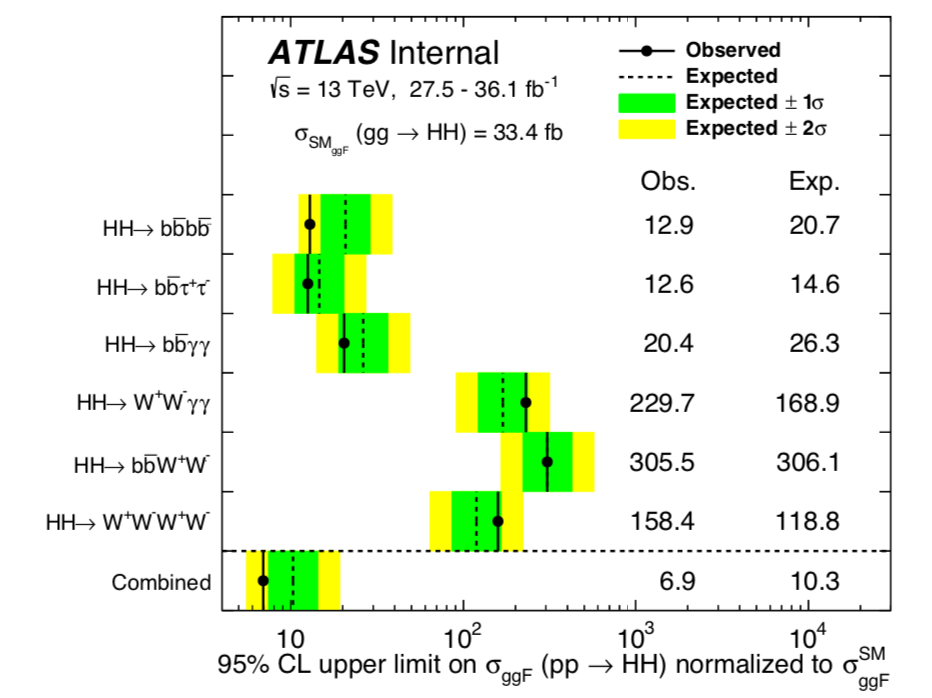
\includegraphics[width=0.75\textwidth]{fig/HH_combined_nonres.png}
 \caption{联合$hh$各衰变道给出的标准模型希格斯对的产生截面上限(归一化到$\sigma_{\text{SM}}$)。}
 \label{fig:HH_combined_nonres}
\end{figure}

\begin{figure}[h]
\centering
 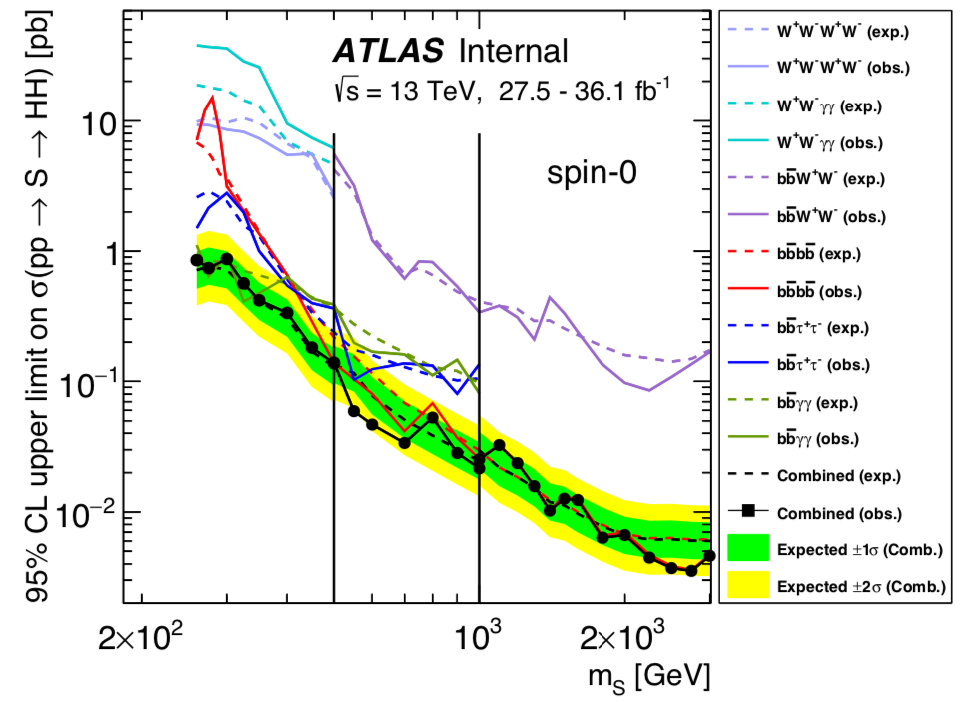
\includegraphics[width=0.75\textwidth]{fig/HH_combined_res.png}
 \caption{联合$hh$各衰变道给出的共振态的产生截面上限(pb)。}
 \label{fig:HH_combined_res}
\end{figure}

在自耦合参数的限定实验中,只考虑了\bbbb , \bbtt 和\bbaa ,因为其他三者贡献不大。
自耦合参数的限定比较复杂,因为信号接收度和形状依赖于$\kappa_{\lambda}$,所以在$\kappa_{\lambda}$的扫描中,对于每个点,一个专门产生的对应该$\kappa_{\lambda}$的信号模板被输入\footnote{考虑到不同$\kappa_{\lambda}$对信号的影响,实际上每个分析道还采用了专门的筛选。},
而后得到$hh$的产生截面上限。每个$\kappa_{\lambda}$点预期截面则根据LHCHXSWG(YR4)\cite{SM-HIGGS-BR}推荐,假设QCD的高阶修正和$\kappa_{\lambda}$修正是可因子化的,在NNLO+NNLL准确性性计算得到一系列随$\kappa_{\lambda}$变化的相对于33.41 fb(即$\kappa_{\lambda}$=1)的修正因子。在上限设置中,每个点的系统误差均采用$\kappa_{\lambda}$=1时的结果。
图\ref{fig:HH_selfcoupling}比较了产生截面上限与理论预期,在95\%置信度下,$\kappa_{\lambda}$的观测(期望)上限在$-5.0<\kappa_{\lambda}<12.1$ ($-5.8<\kappa_{\lambda}<12.0$)内。
\begin{figure}[h]
\centering
 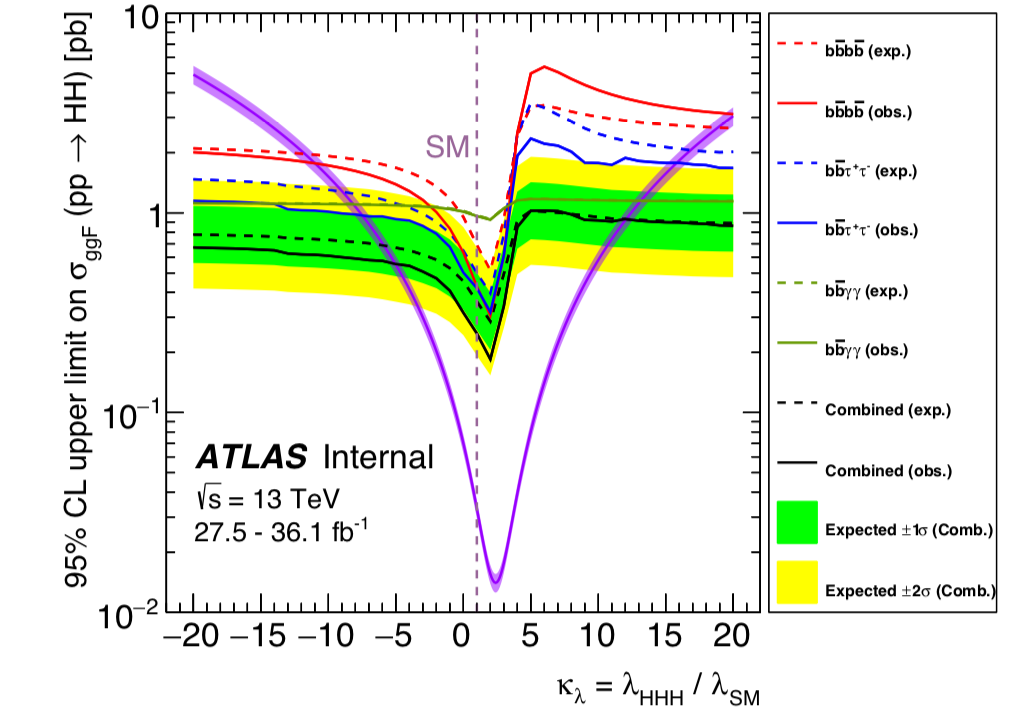
\includegraphics[width=0.75\textwidth]{fig/HH_selfcoupling.png}
 \caption{联合$hh$各衰变道给出的标准模型希格斯对产生截面上限随$\kappa_{\lambda}$变化结果,其中紫色曲线表示理论预期。}
 \label{fig:HH_selfcoupling}
\end{figure}
